% Licensed to the Apache Software Foundation (ASF) under one or more
% contributor license agreements. See the NOTICE file distributed with
% this work for additional information regarding copyright ownership.
% The ASF licenses this file to You under the Apache License, Version 2.0
% (the ``License''); you may not use this file except in compliance with
% the License. You may obtain a copy of the License at
%
% http://www.apache.org/licenses/LICENSE-2.0
%
% Unless required by applicable law or agreed to in writing, software
% distributed under the License is distributed on an ``AS IS'' BASIS,
% WITHOUT WARRANTIES OR CONDITIONS OF ANY KIND, either express or implied.
% See the License for the specific language governing permissions and
% limitations under the License.

\subsubsection{Meridio Job Options}

You must fill in the following extra fields if you are configuring a
Meridio job:

\bigimage{mer-edit-job-tab3}

% Licensed to the Apache Software Foundation (ASF) under one or more
% contributor license agreements. See the NOTICE file distributed with
% this work for additional information regarding copyright ownership.
% The ASF licenses this file to You under the Apache License, Version 2.0
% (the ``License''); you may not use this file except in compliance with
% the License. You may obtain a copy of the License at
%
% http://www.apache.org/licenses/LICENSE-2.0
%
% Unless required by applicable law or agreed to in writing, software
% distributed under the License is distributed on an ``AS IS'' BASIS,
% WITHOUT WARRANTIES OR CONDITIONS OF ANY KIND, either express or implied.
% See the License for the specific language governing permissions and
% limitations under the License.

\begin{itemize}
\label{scheduling}

\item \textbf{Schedule type:} Whether you want to scan every document
once or dynamically recrawl content in your repository. 

When scanning every document once, the crawler marks all documents that
have been previously crawled in this job as potentially to be deleted,
adds all seed documents to its queue and marks them as pending, processes
pending documents, marking them completed as they are ingested, and then
deleted all of the documents that were not recrawled. A document might
not be recrawled because it no longer exists, or the job specification
might have been changed to no longer include the document.

When dynamically recrawling documents, the crawler does not start by
marking all documents as potentially deletable; instead, it begins with
all of the seed documents, and continues adding to its list, periodically
re-adding the initial seed documents. If a document is removed from the
source, it will expire in the expiration interval (see below).

\item \textbf{Expiration Interval (if continuous):} The length of the
interval (in minutes) that the appliance will retain a document
crawled by this job after the document no longer appears in the
repository. After this interval, the missing document will be removed
from the appliance's index and archive. Leave the expiration interval
blank to keep missing documents indexed in GTS.

\item \textbf{Recrawl interval:} If you are dynamically recrawling
documents, how long, in minutes, the crawler should wait before
crawling documents a second time.

\item \textbf{Reseed interval:} If you are dynamically recrawling
documents, how long, in minutes, the crawler should wait before
looking for new documents to crawl. \ifMeridioGuide This connector
identifies all documents for ingestion through seeding; if the reseed
interval is infinite, the job will not ingest documents placed in the
repository during run time. (The job automatically reseeds whenever it
is started.) The default interval of 60 minutes is an appropriate
reseed rate. \fi \ifFilenetGuide This connector identifies documents
for ingestion during seeding. If you change the document inclusion
criteria, reseeding is required to identify new documents. Similarly,
documents placed in the repository while the job is running will not
be identified until the crawl is reseeded.  (The job automatically
reseeds whenever it is started.) The default interval of 60 minutes is
an appropriate reseed rate. \fi

\item \textbf{Scheduled time:} Allows you to define a time you wish
the job to run using a series of selection boxes. The first box refers
to the day of the week you wish the job to run, with an option to have
the job run any day of the week. The second box allows you to select
the start hour, with an option to start the job at any hour. The third
box allows you to specify which minute after the hour that you wish
the job to start. The fourth box allows you to specify what months of
the year you wish the job to run, with an option for the job to run
any month. The last box allows you to specify the day of the month you
wish the job to start, including any day of month.


You can scroll through each of the five boxes in this setting using
the arrow keys on your keyboard or by using the scroll bar on the
right side of the box.  If you want to select more than one value,
hold down control as you scroll and click the values that you want to
select. This allows you to define multiple windows with the same
length, for example by selecting Monday, Wednesday, and Friday at the
same time.

\item \textbf{Maximum run time:} The longest you will allow the job to
run, in minutes. For example, if you want to start a job at 2 AM but
force it to stop at 8 AM so that users have access to the repository,
you should set this value to 360 minutes. If the job is not complete by the
end time, documents that have already been found will be indexed, and
the rest of the crawl will continue at the beginning of the next
schedule interval. 

When you have defined the scheduled time and assigned a maximum run
time, click on the ``Add Scheduled Time'' button. A new schedule box
will appear below the scheduled time, allowing you to create
additional scheduled run times.

Here is a sample schedule for a job that will run every
Monday from 2 am to 6 am:

\begin{changemargin}{-.3in}{0in} 
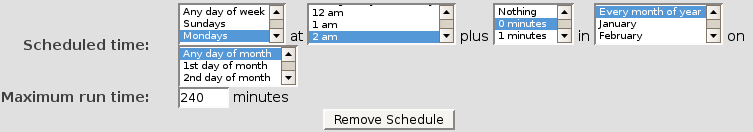
\includegraphics[width=300pt]{sample-schedule}
\end{changemargin}

If you do not have at least one scheduled time, the job will
only run when run manually (see page \pageref{ManageJobs}), and will
not automatically update the index on the appliance based on changes
to the repository.

You can remove a scheduled time by clicking the ``Remove Schedule''
button.

\end{itemize}


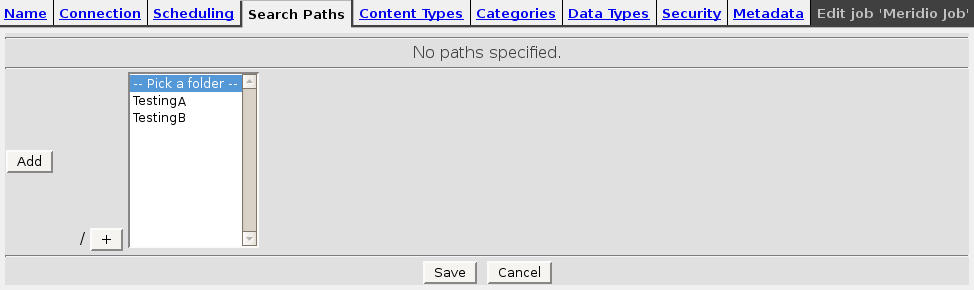
\includegraphics[width=300pt]{mer-edit-job-tab4}

\begin{itemize}

\item \textbf{Paths:} The directory paths in your Meridio
service from which you want your crawl to start. You can specify
one or more directory paths. If you do not specify directory paths,
the job will crawl all directories in your Meridio service. You
can build directory paths by selecting individual directories. To
start, select the base directory of the path you wish to create, then
click the ``+'' button. A new selection box will appear with the
directories contained by that parent directory. Select a directory at
that level and click the ``+'' button. Continue building your
directory path in this fashion. When it's complete, click ``Add''. A
new selection box will appear beneath the added directory path. You
can continue to add more directory paths to your list. To remove a
directory path from the list, click the ``Delete'' button next to it.

\end{itemize}

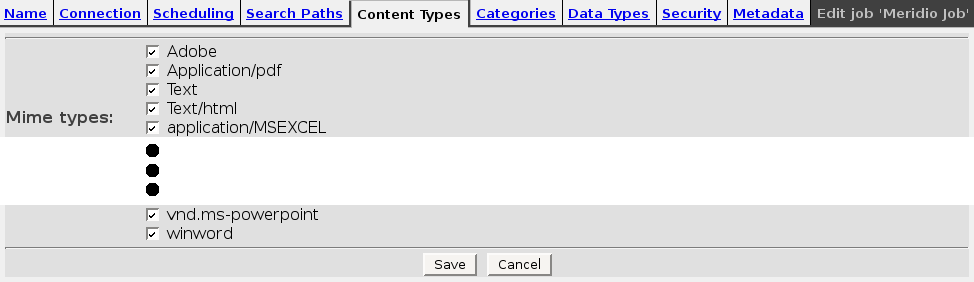
\includegraphics[width=300pt]{mer-edit-job-tab5}

\begin{itemize}

\item \textbf{Mime Types:} Check the
mime types you wish to include in this job. This list of mime types is
based on the mime types that the appliance is capable of ingesting.

\end{itemize}

%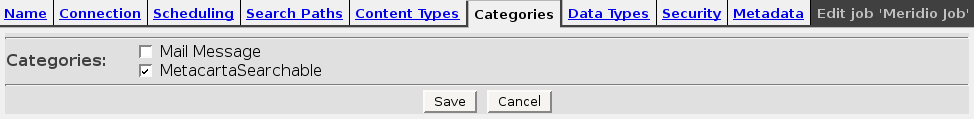
\includegraphics[width=300pt]{mer-edit-job-tab6}

\begin{itemize}

\item \textbf{Categories:} Check the categories that you wish to include in this job. These categories are created by your Meridio administrator; ask your administrator which categories you should include.

\end{itemize}

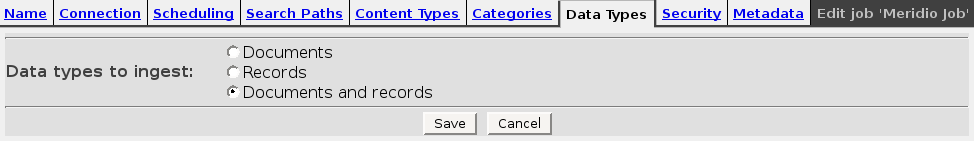
\includegraphics[width=300pt]{mer-edit-job-tab7}

\begin{itemize}

\item \textbf{Data types to ingest:} 
Here you can specify if this job should include \textbf{Documents},
\textbf{Records}, or \textbf{Documents and records}.
 
\end{itemize}


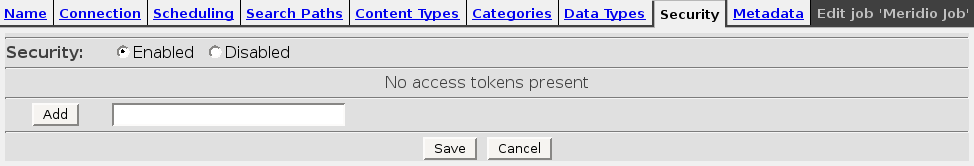
\includegraphics[width=300pt]{mer-edit-job-tab8}

\begin{itemize}

\item \textbf{Security:} Use this option to enable or disable document
security. If you choose to enable security, user permissions will be
ingested with documents, while if you choose to disable security,
documents will be ingested without permissions.

\item \textbf{Access Tokens:} \label{ForceACL} If you wish to specify
your own permissions lists for files ingested through this job, you
can specify them here. You should use this option if you selected
``Standard (Kerberos)'' as the authority connection for your
repository connection and you are choosing to enable security. Simply
enter one or more Meridio user or group identifiers into the field and
click the ``Add'' button. The identifiers will appear in a list. You
can continue to add more identifiers using the ``Add'' button, or
remove them using the ``Delete'' button that appears next to each
identifier.

\end{itemize}

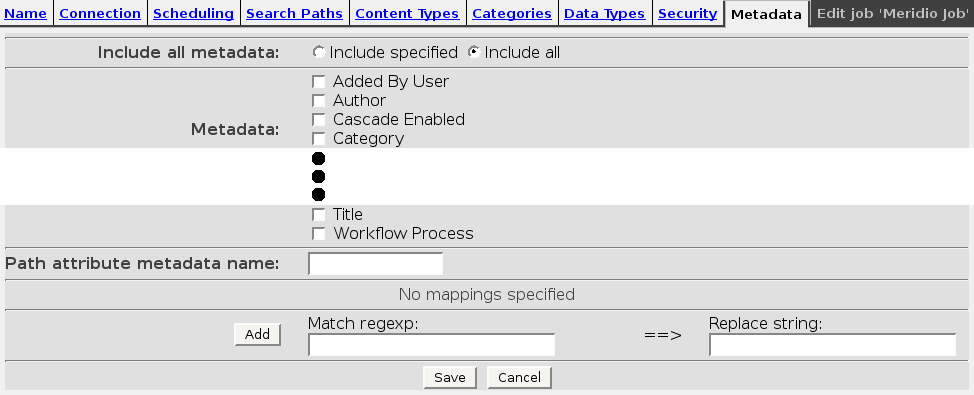
\includegraphics[width=300pt]{mer-edit-job-tab9}

\begin{itemize}

\item \textbf{Include all metadata:} This allows you to chose between including all metadata present for each file and creating a subset of the metadata attributes to include. If you select ``Include specified'', you can use the following field to select the metadata attributes you want to include.

\item \textbf{Metadata:} Each metadata field that is available on your Meridio system is listed here.

\item \textbf{Path attribute metadata name:} The Meridio Connector does not support path attribute metadata. Leave this field blank.

\item \textbf{Path-value mapping:} Leave these fields blank.

\end{itemize}


After entering this information, you will be taken to the status page
for this job:

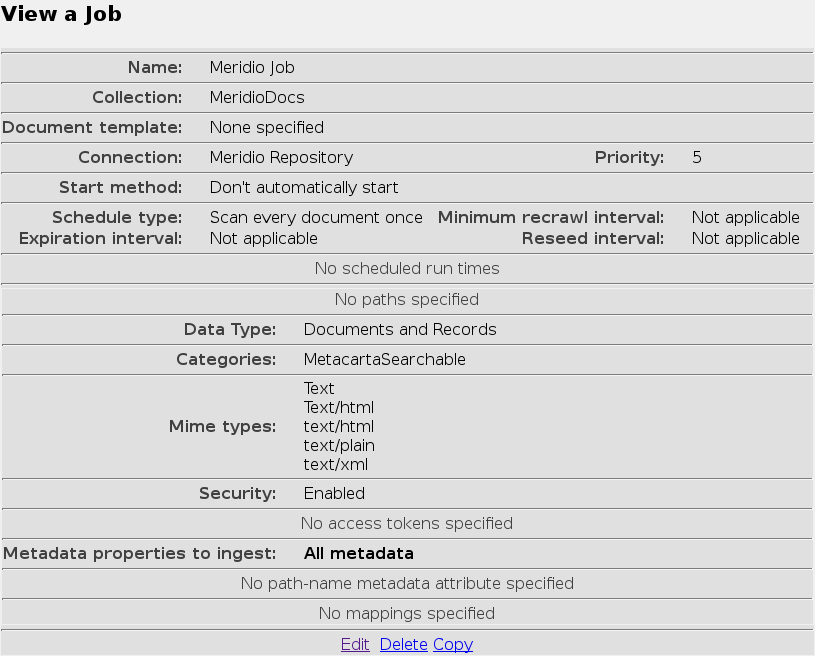
\includegraphics[width=300pt]{mer-view-job-status}

